\documentclass[10pt,conference,a4paper]{IEEEtran}

%
%
%

\usepackage{amsmath, amssymb}
\usepackage{graphicx}
\usepackage[pagebackref=true,breaklinks=true,letterpaper=true,colorlinks,bookmarks=false]{hyperref}
\usepackage{multirow}

\usepackage{authblk}

\usepackage{parskip}
%\usepackage[a4paper, includeheadfoot, margin=1cm]{geometry}

\usepackage{subcaption}

\usepackage{bm}

%
%
%

\usepackage{tikz}
\usepackage{pgfplots}

\DeclareRobustCommand\mydashedrect{\begin{tikzpicture}\draw [red, dotted, line width=1](0,0) -- (.5,0) -- (.5, .25) -- (0, .25) -- cycle; \end{tikzpicture}}
\DeclareRobustCommand\mygreenarrow{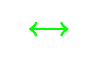
\begin{tikzpicture}\draw [<->, green, line width=1](0, 0.5) -- (0.5, 0.5); \end{tikzpicture}}
\DeclareRobustCommand\myredarrow{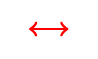
\begin{tikzpicture}\draw [<->, red, line width=1](0, 0.0) -- (0.5, 0.0); \end{tikzpicture}}

\definecolor{darkgreen}{rgb}{0, 0.5, 0}

%
%
%

\begin{document}

	\title
	{
		Learning Local Descriptors by Optimizing the Keypoint-Correspondence Criterion
	}

	\author[$\dagger$]{Nenad Marku\v{s}\thanks{\texttt{nenad.markus@fer.hr}}}
	\author[$\dagger$]{Igor S. Pand\v{z}i\'{c}}
	\author[$\ddagger$]{J\"orgen Ahlberg}
	\affil[$\dagger$]
	{
		\small
		University of Zagreb,
		Faculty of Electrical Engineering and Computing,
		Unska 3, 10000 Zagreb, Croatia
	}
	\affil[$\ddagger$]
	{
		\small
		Computer Vision Laboratory,
		Dept.~of Electrical Engineering,
		Link\"{o}ping University,
		SE-581 83 Link\"{o}ping, Sweden
	}

	\date{}

	\maketitle

	\begin{abstract}
		Current best local descriptors are learned on a large dataset of matching and non-matching keypoint pairs.
		However, data of this kind is not always available since detailed keypoint correspondences can be hard to establish.
		On the other hand, we can often obtain labels for pairs of keypoint bags.
		For example, keypoint bags extracted from two images of the same object under different views form a matching pair, and keypoint bags extracted from images of different objects form a non-matching pair.
		On average, matching pairs should contain more corresponding keypoints than non-matching pairs.
		We describe an end-to-end differentiable architecture that enables the learning of local keypoint descriptors from such weakly-labeled data.
	\end{abstract}

	\section{Introduction}
		Local descriptors are a widely used tool in computer vision and pattern recognition.
		Some example applications include object/scene recognition and retrieval \cite{visualwords,fisherkernel,vlad}, face verification \cite{fisherfaces,localfacerec}, face alignment \cite{sdm}, image stitching \cite{recognisingpanoramas}, 3D shape estimation \cite{shapefrom2dlandmarks} and 3D model retrieval/matching \cite{hybridbow,cov3d}.
		However, despite years of research, there is still room for improvement, as confirmed by recent results based on convolutional neural networks \cite{zagoruyko,matchnet,convdesc,pnnet}.
		Also, we view the research in local descriptors complementary to keypoint detection research, which is still an active area of computer vision (see, for example \cite{tilde}).

		A promising way of obtaining discriminative local descriptors is to learn them from annotated keypoint correspondences.
		This can be used to form a set of matching and non-matching keypoint pairs:
		\begin{equation}\label{eq:kppairs}
			\mathcal{D}_{KP}=
			\{(k_{i1}, k_{i2}, l_i)\}_{i=1}^N
			.
		\end{equation}
		The label $l_i\in\{+1, -1\}$ indicates whether keypoints $k_{i1}$ and $k_{i2}$ form a matching or a non-matching pair.
		See \cite{brown,binboost,rfd,zagoruyko,matchnet,convdesc} for some recent examples of descriptor learning methods that use data in this form.
		Another possibility is to form a set of keypoint triplets:
		\begin{equation}\label{eq:kptriplets}
			\mathcal{D}_{KT}=
			\{(k_i, k_i^+, k_i^-)\}_{i=1}^N
			,
		\end{equation}
		where $k_i$ and $k_i^+$ match and $k_i$ and $k_i^-$ do not.
		Balntas et al. \cite{pnnet} use data in this form in their method.
		The standard dataset for learning and benchmarking various image keypoint descriptors was introduced by Brown et al. \cite{brown}. %: \url{http://www.cs.ubc.ca/~mbrown/patchdata/patchdata.html}.
		It contains around $1.5$M patches cropped around difference of Gaussians keypoints \cite{sift} obtained from multiple views of three different scenes: the Notre Dame Cathedral, the Statue of Liberty and the Yosemite Half Dome.
		High-quality keypoint labels were obtained with a multi-view stereo algorithm \cite{multiviewstereo}.
		This makes the dataset reliable both for learning local image-patch descriptors from "handcrafted" features \cite{cvx,binboost,rfd} and large models based on convolutional neural networks \cite{osendorfer,zagoruyko,matchnet,fracking,convdesc,pnnet}
		(the siamese-network framework of Hadsell et al. \cite{siamesenet}).
		However, in the general case, this kind of data is relatively hard to obtain, even more so for non-image data (e.g., 3D models, depth maps, voxel data, video signals, etc.).

		Instead of having a dataset with individual keypoint correspondences (which lead to dataset types \eqref{eq:kppairs} and \eqref{eq:kptriplets}) for learning local descriptors as in most prior work, we assume a set of labeled \emph{bags of keypoints}
		(here we intentionally use the terminology from multiple instance learning \cite{MIL} as our ideas are closely related with the field).
		We denote this weakly-labeled dataset as
		\begin{equation}\label{eq:bagtriplets}
			\mathcal{D}_{BT}=
			\{(K_{i}, K_i^+, K_i^-)\}_{i=1}^N
			,
		\end{equation}
		where bags $K_i$ and $K_i^+$ form a matching pair, bags $K_i$ and $K_i^-$ form a non-matching pair, and each bag is a set of $n$ keypoints, $K=\{k_1, k_2, \ldots, k_n\}$.
		Data of this kind is relatively easy to generate.
		For example, keypoint bags extracted from two images of the same object under different views form a matching pair.
		These bags can be used together with a keypoint bag extracted from an image of some unrelated object to form a triplet from Equation \eqref{eq:bagtriplets}.
		See Figure \ref{fig:teaser} for an illustration.
		\input{teaser.fig}
		This paper describes a method for learning local descriptors from such weakly-labeled data.

	\section{Related work}
		We already mentioned a large body of work in local image descriptors and we will not repeat these standard approaches in this section.

		We would like to explicitly mention the work of Paulin et al. \cite{kernelconv} since they are also motivated to obtain discriminative local descriptors by means that do not require strongly-labeled data (equations \eqref{eq:kppairs} and \eqref{eq:kptriplets}).
		To achieve their goal, they adapt the convolutional kernel network approach, which is an unsupervised framework for learning convolutional architectures \cite{kernelconv0}.

		The learning procedure we propose in the next section is related to the one by Arandjelovi\'{c} et al. \cite{netvlad}, as they also propose to learn descriptors from weakly-labeled data.
		Unlike us, they do not focus on local descriptors and learn whole image representations instead.
		Also, they derive their learning procedure from a different perspective: we are concerned with local image correspondences and how to find them, and they focus on learning a global descriptor for image retrieval.
		It is not clear how well would their system work in finding local correspondences between two images.
		Also, we learn our descriptors \textit{directly} for comparisons with $L_2$ distance.

	\section{Method}\label{sec:core}
		We study how to the learn parameters of a descriptor extraction process that transforms a local neighborhood of a keypoint (e.g, a patch extracted around a distinctive corner within an image) into a short vector in such a way that similar keypoints are "close" and dissimilar keypoints are "far".
		Two attractive properties of such representations are low memory requirements and fast matching times.
		Unlike most prior work, our learning method exploits the information in weakly-labeled data to achieve mentioned goals.

		In this paper, we denote the descriptor extraction process as $e$ (this is basically a number of predefined computational steps).
		For example, in our experiments, $e$ is a convolutional neural network (see Table \ref{tbl:nn} for its architecture) that maps a $32\times 32$ local image patch into a $64$-dimensional vector.
		We denote the parameters of $e$ as $\theta_e$.
		Here we describe an effective procedure for learning $\theta_e$ from the training data given by Equation \eqref{eq:bagtriplets}.
		First, we define that two keypoints match if the $L_2$ distance between their signatures (extracted by $e$) is less than or equal to some threshold $\tau\in\mathbb{R}$.
		This threshold is a parameter of the learning process and we specify some recommended values later in the text.
		Next, we define a \emph{matching score} between two bags of keypoints (both of size $n$), $K_1$ and $K_2$, as
		\begin{equation}\label{eq:bagsim}
			S_{e, \tau}(K_1, K_2)=
			\frac{m_{e, \tau}(K_1, K_2)}{n}
			,
		\end{equation}
		where $m_{e, \tau}(K_1, K_2)$ is the number of keypoints from $K_1$ that have a matching keypoint in $K_2$ for the descriptor extractor $e$ and threshold $\tau$.
		Optimal matching could be computed with the Hungarian algorithm in $O(n^3)$ time.
		However, this is too slow in our case and we use the following $O(n^2)$ approximation
		(inspired by the "sum-max" match kernel from \cite{summax}):
		$$
			m_{e, \tau}(K_1, K_2)=
			\sum_{i=1}^n \left[ \min_{j=1}^n d_{ij}^2 \leq \tau \right]
			,
		$$
		where $[\;\cdot\;]$ represents the indicator function\footnote{$[p]=1$ if the proposition $p$ is true and $[p]=0$ otherwise.} and $d_{ij}$ is the Euclidean distance between descriptors of $k_i\in K_1$ and $k_j\in K_2$, i.e.,
		$$
			d_{ij} =
			|| e(k_i) - e(k_j) ||_2
			.
		$$
		We want high $S_{e, \tau}$ for matching bags and low $S_{e, \tau}$ for non-matching bags.
		Thus, a suitable loss for parameter learning is
		\begin{equation}\label{eq:loss}
			L=
			\sum\frac{S_{e, \tau}(K, K^-)}{S_{e, \tau}(K, K^+) + \epsilon}
			,
		\end{equation}
		where the summation goes over $(K, K^+, K^-)\in\mathcal{D}_{BT}$ (Equation \eqref{eq:bagtriplets}) and $\epsilon$ is a small constant included for numerical stability.
		However, since $S_{e, \tau}$ is not continuous, we cannot apply the standard gradient-based learning techniques.
		Thus, we resort to the following approximation of the function $[x\leq\tau]$ for $x\in\mathbb{R}$:
		$$
			[x\leq\tau]\approx
			\frac{1}{1 + \exp(\beta(x-\tau))}
			,
		$$
		where the parameter $\beta$ regulates the "strength" of the approximation.
		Since the loss function $L$ is now differentiable, the parameters $\theta_e$ can be tuned with standard backpropagation-based methods.
		However, as we cannot optimize the proposed criterion (i.e., find its global minimum), we approximate the solution with a local minimum to which the learning converges and experimentally show that this leads to good results.

		To simplify the implementation, we require that the extractor outputs descriptors of unit length: $||e(k_i)||_2=||e(k_j)||_2=1$.
		Notice that in this scenario
		$$
			d_{ij}^2=
			|| e(k_i) - e(k_j) ||_2^2 =
			2 - 2e(k_i)^Te(k_j)
		$$
		and the matching score function $S_{e, \tau}$ (Equation \eqref{eq:bagsim}) depends only on the matrix $\mathbf{S}\in\mathbb{R}^{n\times n}$ computed as
		$$
			\mathbf{S}=
			\mathbf{E}_1\mathbf{E}_2^T
			,
		$$
		where the rows of matrices $\mathbf{E}_1$ and $\mathbf{E}_2$ contain descriptors extracted with the extractor $e$ from keypoints in $K_1$ and $K_2$.
		The backpropagation expressions are quite elegant in this setting:
		\begin{align*}
			\frac{\partial S_{e, \tau}(K_1, K_2)}{\partial \mathbf{E}_1}&=\frac{\partial S_{e, \tau}(K_1, K_2)}{\partial \mathbf{S}}\cdot\mathbf{E}_2	\\
			\frac{\partial S_{e, \tau}(K_1, K_2)}{\partial \mathbf{E}_2}&=\left(\frac{\partial S_{e, \tau}(K_1, K_2)}{\partial \mathbf{S}}\right)^T\cdot\mathbf{E}_1
		\end{align*}
		where $\partial S_{e, \tau}(K_1, K_2)/\partial \mathbf{S}$ is straightforward to compute because $S_{e, \tau}$ contains only the standard components usually used in neural networks (see the definition, Equation \eqref{eq:bagsim}).
		The proposed computational steps can be implemented very efficiently in just a few hundred lines of Torch7 code.
		Another advantage of unit-length descriptors is that this greatly simplifies the selection of the threshold $\tau$ because the Euclidean distance between two descriptors falls in the $[0, 2]$ interval.

		The next section provides experiments which show that the proposed learning procedure leads to good results.

	\section{Experiments}
		We perform experiments with image patch descriptors extracted around local detected keypoints.
		We use the following datasets to provide numerical evidence for our observations:
		\begin{itemize}
			\item
				UKB \cite{ukb} ($2500$ objects, $4$ views each);
			\item
				ZuBuD \cite{zubud} ($200$ buildings, $5$ images each);
			\item
				INRIA Holidays \cite{holidays}
				(approximately $1500$ images of $500$ different scenes).
		\end{itemize}
		See Figure \ref{fig:databases} for some examples.
		\begin{figure*}
			\centering
			\resizebox{1.975\columnwidth}{!}
			{
				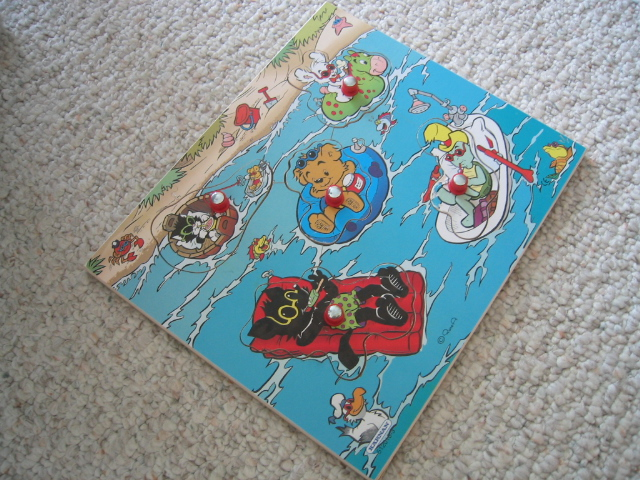
\includegraphics[scale=0.091]{ukbench00000.jpg}
				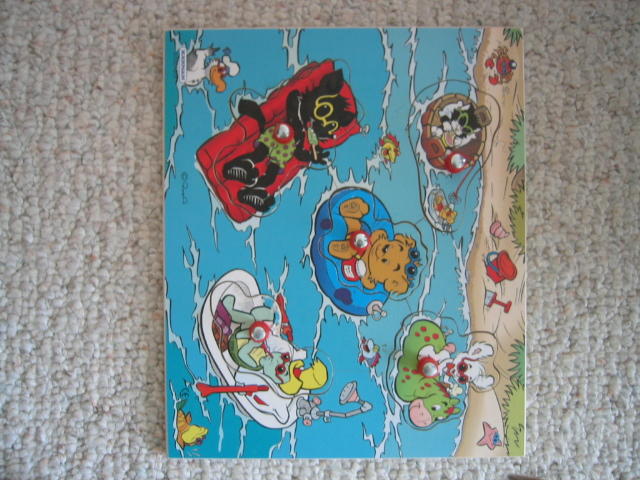
\includegraphics[scale=0.091]{ukbench00002.jpg}
				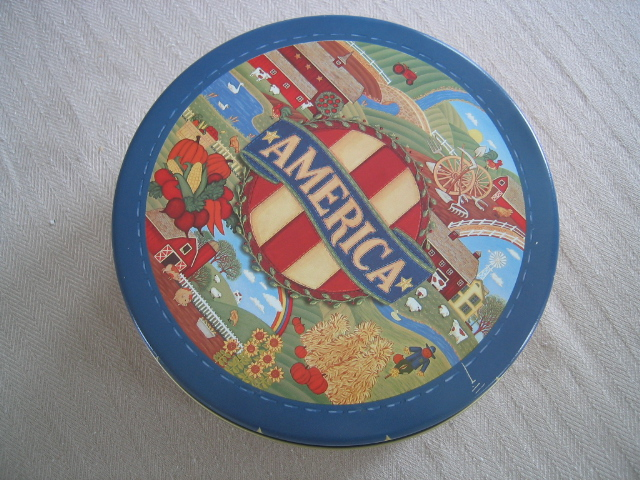
\includegraphics[scale=0.091]{ukbench00005.jpg}
				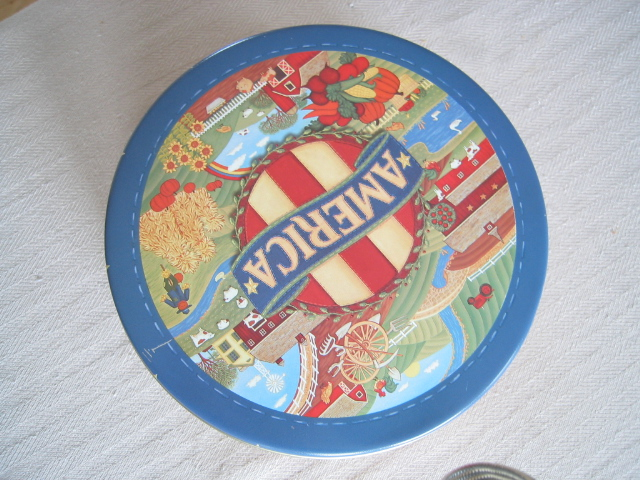
\includegraphics[scale=0.091]{ukbench00006.jpg}
				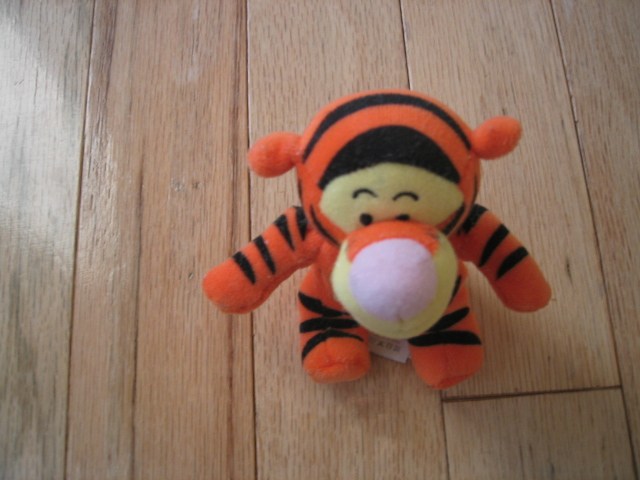
\includegraphics[scale=0.091]{ukbench03810.jpg}
				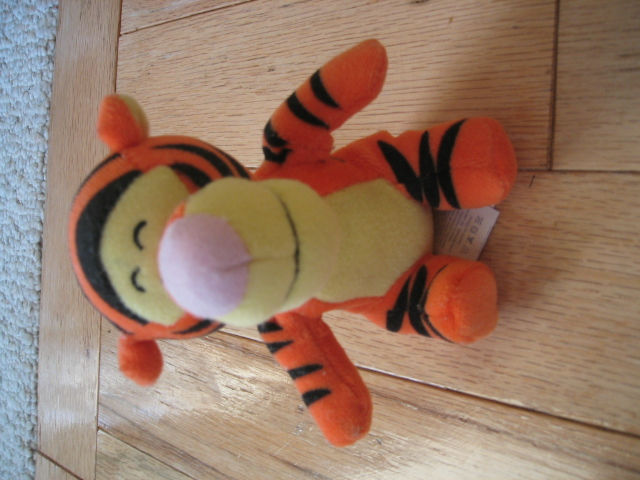
\includegraphics[scale=0.091]{ukbench03811.jpg}
				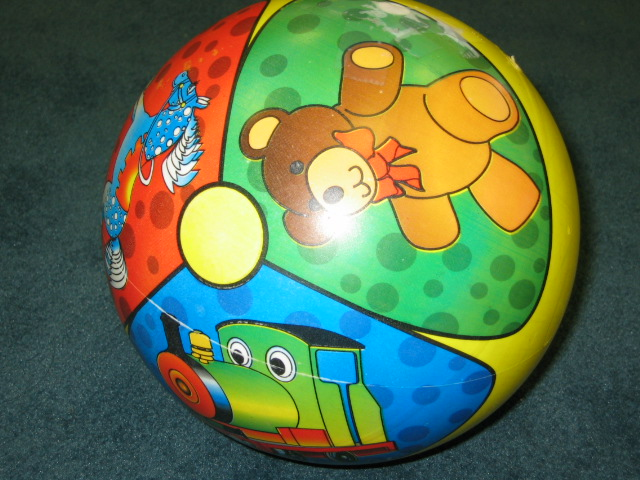
\includegraphics[scale=0.091]{ukbench09985.jpg}
				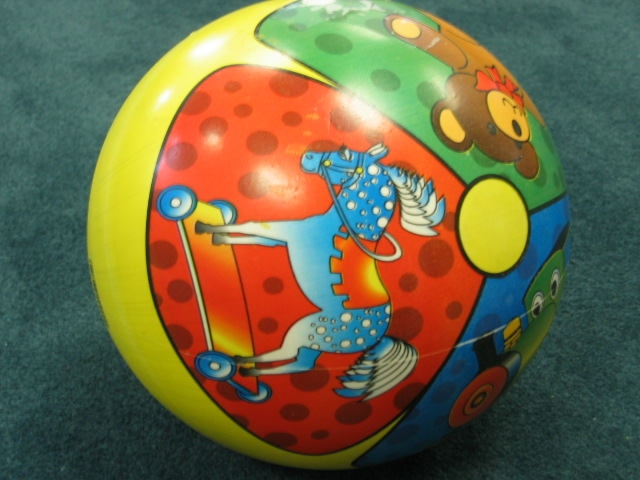
\includegraphics[scale=0.091]{ukbench09987.jpg}
			}

			\resizebox{1.975\columnwidth}{!}
			{
				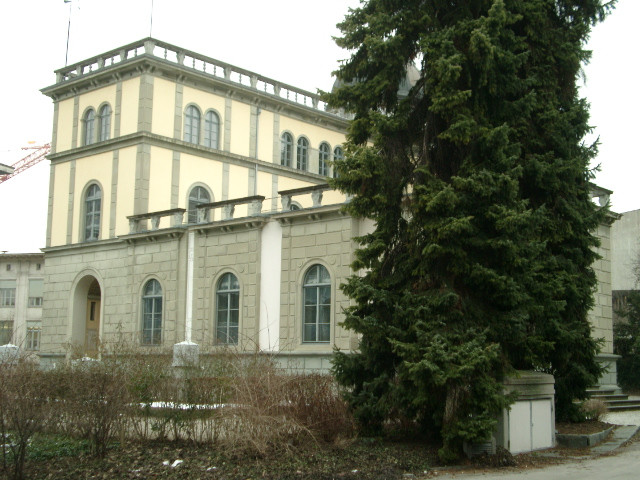
\includegraphics[scale=0.123]{zubud1.jpg}
				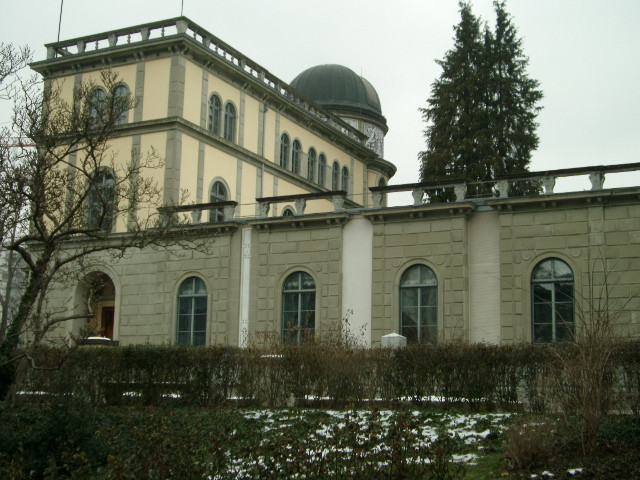
\includegraphics[scale=0.123]{zubud2.jpg}
				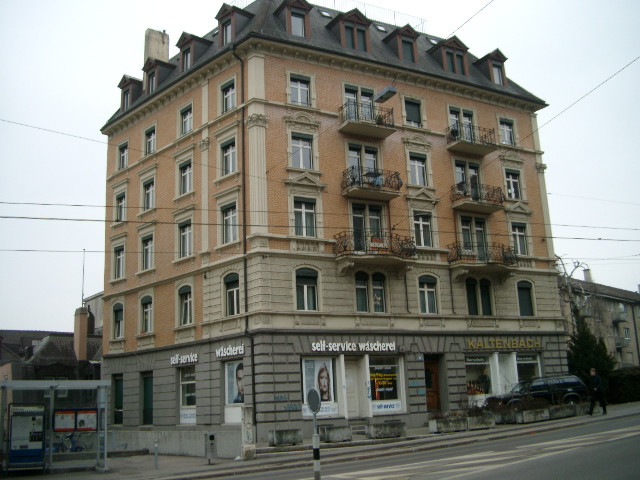
\includegraphics[scale=0.123]{zubud3.jpg}
				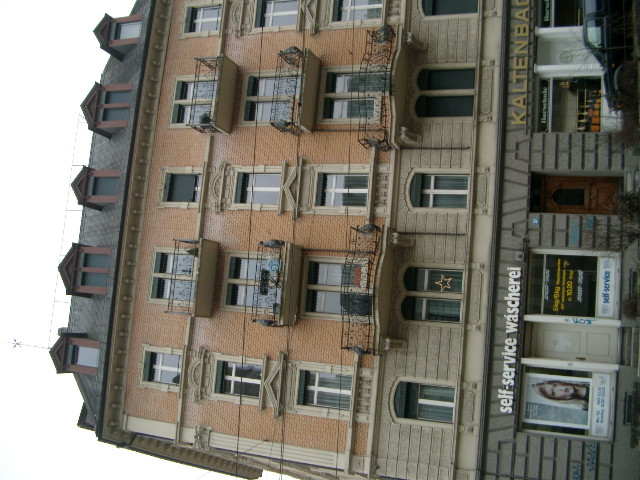
\includegraphics[scale=0.123]{zubud4.jpg}
				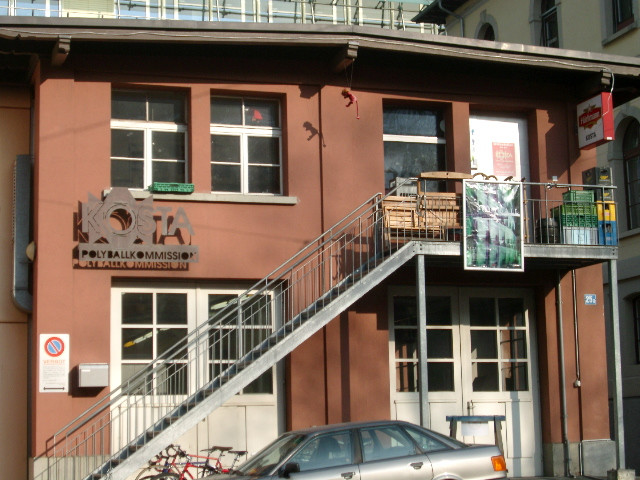
\includegraphics[scale=0.123]{zubud5.jpg}
				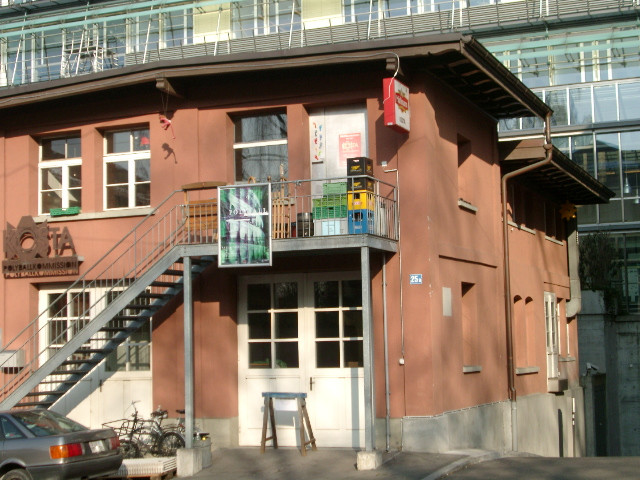
\includegraphics[scale=0.123]{zubud6.jpg}
			}

			\resizebox{1.975\columnwidth}{!}
			{
				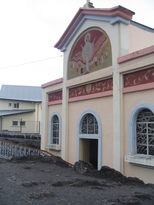
\includegraphics[scale=0.82]{inria1.jpg}
				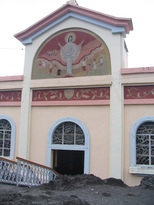
\includegraphics[scale=0.82]{inria2.jpg}
				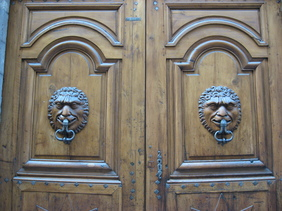
\includegraphics[scale=0.82]{inria3.jpg}
				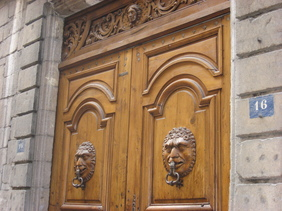
\includegraphics[scale=0.82]{inria4.jpg}
				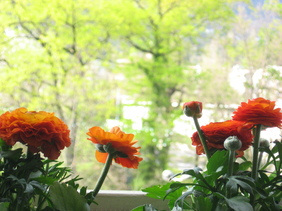
\includegraphics[scale=0.82]{inria5.jpg}
				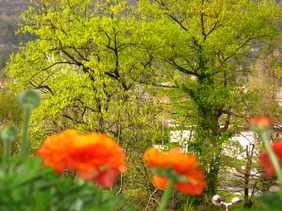
\includegraphics[scale=0.82]{inria6.jpg}
			}

			\caption
			{
				Samples from databases used in our experiments:
				UKB \cite{ukb} (first row),
				ZuBuD \cite{zubud} (second row),
				INRIA Holidays \cite{holidays} (third row).
			}
			\label{fig:databases}
		\end{figure*}

		In our experiments, each image is downsampled by a factor of four to reduce noise, filter out irrelevant content and increase keypoint stability.
		Next, image patches are extracted around detected keypoints.
		These steps set up a basis for a fair comparison between different descriptors since we always use the same keypoints
		(location, size\footnote{A patch of a fixed size around the keypoint is resampled to $32\times 32$ or $64\times 64$ pixels, depending on the requirements of the method.} and orientation).

		\subsection{Learning convolutional features with our method}
			The architecture of our neural network-based descriptor extractor $e$ can be seen in Table \ref{tbl:nn}.
			\begin{table}
				\resizebox{\columnwidth}{!}
				{
				\begin{tabular}{|c||c|c|c|c|}
					\hline
					Conv. layer	&	1	&	2	&	3	&	4	\\
					\hline
					\hline
					Filter size	&	$3\times 3$	&	$4\times 4$	&	$3\times 3$	&	$1\times 1$	\\
					\hline
					Stride	&	1	&	2	&	1	&	1	\\
					\hline
					Output channels	&	32	&	64	&	128	&	32	\\
					\hline
					Activation function	&	ReLU	&	ReLU	&	None	&	None	\\
					\hline
					Max pooling?	& No	&	No	&	Yes, $2\times2$	&	No	\\
					\hline
				\end{tabular}
				}
				\caption
				{
					Our descriptor extractor is a fairly simple convolutional neural network that maps a $32\times 32$ RGB patch into a $64$-dimensional vector.
					It consists of four convolutional layers (given in table above), a fully connected layer that maps the output of the last convolutional layer to $64$ neurons and a final $L_2$ normalization module (i.e., the output vector has unit length).
					The network has around $180$k parameters.
				}
				\label{tbl:nn}
			\end{table}
			To generate the training data for our method, we partition the keypoint bags extracted from the UKB dataset into two subsets.
			The larger subset contains 2200 objects and is used to sample keypoint bag triplets.
			This subset is used for learning and the rest of the UKB dataset (300 objects) is used for validation and testing.
			We train each of our networks for 128 rounds.
			Each round starts by sampling approximately 5000 random $(K, K^+, K^-)$ triplets from the training dataset and loading them onto the GPU.
			These triplets are then used in a standard mini-batch learning for 512 iterations of \texttt{rmsprop}:
			we approximate the loss function $L$ (Equation \eqref{eq:loss}) with a subset of $32$ randomly selected triplets.
			After each round has finished, we test the performance of the network on the validation dataset.
			If the validation loss does not decrease for several rounds, the learning rate is halved.
			The initial learning rate of $0.001$ works good for mini-batches of size 32.
			Also, we set $\epsilon=10^{-6}$, $\beta=20$ and $\tau=0.8$
			(however, it seems that the method is not particularly sensitive to any of these values).
			The total learning time in this setting is approximately one day on a GeForce GTX 970 GPU with cuDNN.
			See Figure \ref{fig:trnprogress} for a typical behavior of average loss ($L$ from Equation \eqref{eq:loss} divided by the number of triplets) throughout the learning process.
			\begin{figure}
				\centering
				\resizebox{1\columnwidth}{!}
				{
					\input{trn.plot}
				}
				\caption
				{
					Typical behavior of the learning process on the UKB training and validation subsets.
				}
				\label{fig:trnprogress}
			\end{figure}

			We learn two models with the same architectures and learning parameters, as described in the previous paragraph.
			The difference between these models were the keypoints.
			The first model is learned on patches extracted with the FAST keypoint detector ($75$ per image).
			The second model combines both FAST and DoG keypoints ($75+75$ per image).

			In the next section we present a comparison of some recently introduced local descriptors.

		\subsection{Matching-based retrieval}
			Following \cite{rfd}, we implement a simple visual search engine to compare the discriminative power of different descriptors.
			The retrieval  is  based  on  the number of matching keypoints between the query and database images ($S_{d, \tau}(K_1, K_2)$, see Equation \eqref{eq:bagsim} for the definition).
			The threshold $\tau$ is tuned separately for each descriptor to produce the best possible results (we simply try all reasonable values; note that this is fair since all descriptors get the same treatment \cite{rfd}).
			We assume that improvements in feature detection and aggregation would benefit all descriptors equally, without changing the relative performance differences.
			This is a common assumption needed to keep the experimentation time reasonable; see, for example, \cite{kernelconv}.
			We benchmark the retrieval performance with the nearest neighbor (NN), first tier (FT) and second tier (ST) scores.
			The idea is to check the ratio of retrieved objects in the query's class that also appear within the top $k$ matches.
			Specifically, for a class with $C$ members, $k=1$ for NN, $k=C-1$ for FT and $k=2(C-1)$ for ST.
			The final score is an average over all the objects in the database.

			For competing neural network-based descriptors, we download the models provided by the authors and apply PCA when necessary
			(e.g., to reduce decriptor size to a more manageable dimensionality).
			Also, note that the binary descriptors are compared with the Hamming distance.

			Tables \ref{tbl:cmpfast} and \ref{tbl:cmpdog} contain the retrieval results for various competing approaches.
			\input{cmp.tbl}
			The descriptor learned with our method (first two rows of both tables) obtain best results on average.
			The difference is particularly significant when compared to "handcrafted" features.
			When comparing the retrieval scores of our two models, it seems that tuning the performance for a particular patch-appearance distribution (i.e., the keypoint detector) leads to a non-negligible difference.
			The model learned on FAST keypoints performs slightly better on the FAST benchmark (Table \ref{tbl:cmpfast}) than the model learned on both DoG and FAST keypoints.
			A possible explanation is that a part of the representational power of the network is expended for representing blob-like DoG features.
			It is the other way arround on the DoG benchmark (Table \ref{tbl:cmpdog}).
			Note that the experiments presented so far measure how well do the descriptors recognize individual keypoints (a useful property for, e.g., object pose recognition).
			Our descriptors are \textit{tuned} for this kind of matching-based recognition task and it would be interesting to see how they perform on some other task.

		\subsection{VLAD-based retrieval}
			In this subsection we experiment with image retrieval based on local feature aggregation.
			Note that none of the descriptors were tuned specifically for this task.
			For each image, we transform approximately $1000$ SURF \cite{surf} keypoints into descriptors and encode them with VLAD \cite{vlad} (a simplified Fisher kernel representation \cite{fisherkernel}).
			The centroids were generated with $k$-means on a subset of images.
			The similarity between two images is measured by an inner product between their VLADs.
			Figure \ref{fig:vlad} shows the NN, FT and ST retrieval scores on three datasets for different local descriptors
			(from our models, we show only the one trained on FAST keypoints because both achieve approximately the same scores in these experiments).
			\begin{figure*}[ht]
				\centering
				\resizebox{1.99\columnwidth}{!}
				{
					\input{ukb-vlad.plot}
				}
				\resizebox{1.99\columnwidth}{!}
				{
					\input{zubud-vlad.plot}
				}
				\resizebox{1.99\columnwidth}{!}
				{
					\input{holidays-vlad.plot}
				}
				\caption
				{
					VLAD-based retrieval results on the UKB-test (first row), ZuBuD (second row) and INRIA Holidays (third row) datasets for varying number of centroids generated with $k$-means.
					The legend for all graphs is plotted in the top-left one.
					The VLAD size is the product of the local descriptor size and the number of centroids.
				}
				\label{fig:vlad}
			\end{figure*}
			We see that our approach leads to results as good as or superior to the so far best published methods and significantly outperforms SIFT (which serves as a baseline).

	\section{Conclusion}
		We point out that the current best methods for learning local descriptors require a large number of matching and non-matching keypoint pairs.
		Data of this kind is not always available and, thus, these methods are not always applicable.
		To address this issue, we introduce a novel algorithm for learning local descriptors from weakly-labeled datasets.
		Experimental results show that our descriptors compare well to the best available ones.
		The code and the learned models can be obtained from \url{https://github.com/nenadmarkus/wlrn}. %(online since February 2016).

	\section*{Acknowledgements}
	%\textbf{Acknowledgements.}
	This research was partially supported by Visage Technologies AB (Link\"oping, Sweden), and by the Croatian Science Foundation (project 8065).

	%\small
	%\bibliographystyle{plain}
	\bibliographystyle{IEEEtran}
	\bibliography{references}

\end{document}